\chapter{L'inversion de formes d'onde}

\section{ce que c'est}

\section{Problème direct}
formulation forte ou faible : 
FDTD, FEM,...

\section{Optimisation}

\subsection{Acoustique isotrope}
\subsection{Acoustique VTI}




\section{application au cnd de soudure : les problématiques}

-guide d'onde
-acquisition en surface seulement, et problématique de la soudure bombée
-anisotropie (cf image soudure) forte, qui touche not. les ondes S.
-acquisition horizontale pas idéale pour inverser la vitesse horizontale (car petits offsets et peu de courbure de rayon comme en géophys)
-sources et récepteurs mobiles 
-geophysique, dispositif de surface, donc on ne considère que les diffractions rayonnant vers la surface (soit angle de diffraction de max 180°)(Forgues, pages 160). En CND, on illumine des deux côté


\begin{figure}
	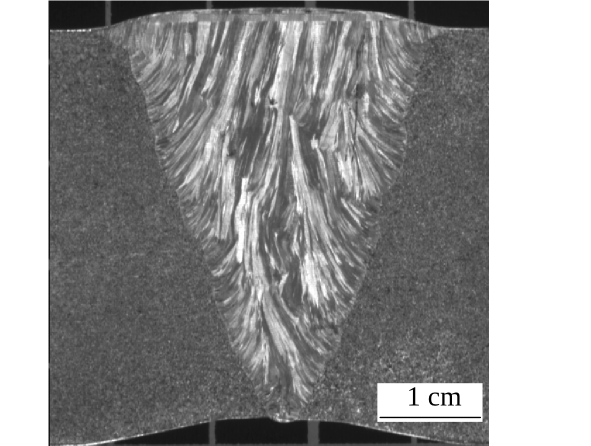
\includegraphics[height=5cm]{./img/soudure1.png}
	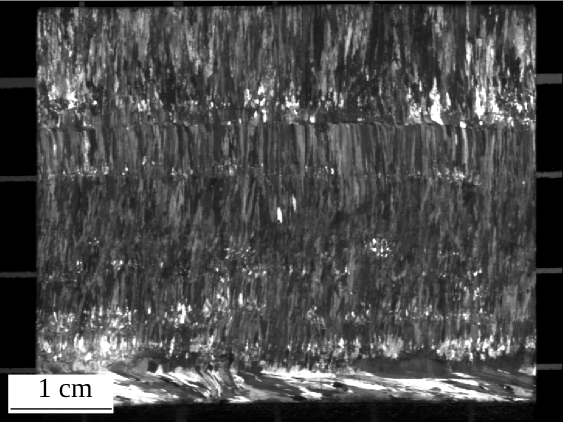
\includegraphics[height=5cm]{./img/soudure2.png}
	\caption{Macrographie d'une soudure industrielle en acier inoxydable en acier austénitique \citep{chassignole}. À gauche : coupe dans le plan $(x,z)$, à droite : coupe dans le plan $(x,y)$.}
\end{figure}
\todo[inline]{préciser les plans sur un schéma et l'orientation des photos}

grains colonnaires
